% !TEX root = ../intro-stellar-physics.tex

Computing is now ubiquitous in science and technology, and is a ``third leg'' along with theory and experiment. Stellar modeling has a long and storied history in this area. Of course, libraries of numerical routines are now widely available, and for research it is far better to use a well-written and well-tested routine than trying to build your own. One still needs to have a basic understanding, however, of how a computational technique works! In this appendix, we wish to give a flavor of a few common numerical techniques. 

\section{Numerical precision}\label{s.numerical-precision}
Before diving into the sea of computational techniques, we need to wade a bit in the shallows of floating-point arithmetic. Numbers are stored in base-2 (binary) format: a sequence of 1's and 0's known as \newterm{bits}. Because the number of bits is finite\sidenote{On most systems the default is 64 bits.}, not all numbers are representable and the processor and compiler define a particular model to represent numbers.

In symbols, an integer $d$ can be written, using $N$ bits, as
\[
d = s\times\sum_{k=1}^{N-1} d_{k}2^{k-1}.
\]
Here $s=\pm1$ is the \newterm{sign bit} and $d_{k} = 0,1$. The largest integer in this representation is $2^{N-1}-1$. For example, suppose we are using $N=4$ bits; one bit is reserved to indicate the sign, and with the remaining 3 bits we represent the positive integers from $0$ to $2^{4-1}-1 = 7$ as
\begin{tabular}{rrrrrrrr}
0 & 1 & 2 & 3 & 4 & 5 & 6 & 7\\
\hline
000 & 001 & 010 & 011 & 100 & 101 & 110 & 111
\end{tabular}.

Real numbers can be modeled in base-2 as follows\cite{Metcalf2018Modern-Fortran-}: for $x \neq 0$, 
\begin{equation}\label{e.modal-reals}
x = s\times 2^{\varepsilon}\times \sum_{k=1}^{p} f_{k}\times 2^{-k}.
\end{equation}
Here the exponent $\varepsilon_{\min}\le\varepsilon\le\varepsilon_{\max}$ and $f_{k}=0,1$ with $f_{1} = 1$.\marginnote{The IEEE 754 64-bit model uses 11 bits for representing the exponent $\varepsilon$ and the remaining 53, including the sign bit $s$, for the fractional part, known as the \newterm{mantissa}. Other common models include 32 bits (8 for exponent, 24 for mantissa) and 128 bits (15 for exponent, 113 for mantissa).} For example, if $\varepsilon=-6$ and $f_{k} = 11010000\ldots$ (i.e., $f_{k}=1$ for $k=\{1,2,4\}$), then
$x = 2^{-6}\times (2^{-1}+2^{-2}+2^{-4}) = 0.0126953125$.

Using the numerical inquiry functions in Fortran 2018, I wrote a small program to report on the arithmetic on my MacBook Pro (Intel Core i5 processor) for 64-bit floating-point arithmetic. The results are as follows.
\begin{Verbatim}[numbers=none]
     exponent = [-1021, 1024]
 [tiny, huge] = [ 2.2251E-308, 1.7977E+308]
    precision = 15
      epsilon = 2.2204E-16
\end{Verbatim}
Let's understand what these numbers mean.
First, the exponent ranges over $-1021\le\varepsilon\le1024$;%
\marginnote{If you are counting, it may seem that $\varepsilon_{\min}$ should be -1023; however, a couple special values of $\varepsilon$ are reserved to indicate exceptions: \texttt{NaN} (not a number), e.g., $\sqrt{-1}$; $\pm$\texttt{Infinity}, e.g., $1/0$; or underflow---the number is too small to be represented in this model with $f_{1}=1$.}
given this, the smallest positive number (with $f_{1}=1$) that can be represented by the model (eq.~[\ref{e.modal-reals}]) has $\varepsilon = \varepsilon_{\min}$ and $f_{k\neq 1} = 0$:
\[\mathtt{tiny} = 2^{\varepsilon_{\min}}\times 2^{-1} = 2^{-1022} = \sci{2.2251}{-308}.\]
The largest positive number that can be represented with eq.~(\ref{e.modal-reals}) is found by setting $\varepsilon=\varepsilon_{\max}$ and all $f_{k}=1$:
\marginnote{In this expression use the formula for the sum of the geometric series,
\[
\sum_{k=1}^{p}r^{-k} = \frac{1-r^{-p}}{r-1}
\]
with $r=2$.}
\[
\mathtt{huge} = 2^{\varepsilon_{\max}}\times \sum_{k=1}^{p} 2^{-k} = 2^{\varepsilon_{\max}}\times(1-2^{-p}) = \sci{1.7977}{308}.
\]
Finally, we can ask: what is the smallest number that, when added to one, gives a number different than one? The number one is represented with $\varepsilon = 1$ and $f_{k} = 10000\ldots$, i.e., $f_{1}=1$ and $f_{k\neq1}=0$. The next number larger than one that can be represented in the model (eq.~[\ref{e.modal-reals}]) has $f_{k} = 10000\ldots00001$; that is, $f_{1}=f_{p}=1$ and all other $f_{k}=0$. Hence, the smallest difference between two real numbers that we can model with eq.~(\ref{e.modal-reals}) is $\mathtt{epsilon} = 2^{-p} = 2^{-52} = \sci{2.2204}{-16}$; our \verb+precision+ is therefore about 15 digits in decimal format.

\section{Finding the root of a function}
A common task in computation is to find the root of a function: that is, given a function $f(x)$ defined on an interval $a\le x\le b$ with $f(a)$ and $f(b)$ having opposite signs, find $x_{r}\in[a,b]$ such that $f(x_{r}) = 0$.
For example, suppose we want to find the root for the function $f(x) = x^2-2$ with $x > 0$. That is, we want to find $r > 0$ such that $f(x=r) = 0$. Of course, the answer has an algebraic solution, namely $\sqrt{2}$ so we don't need to find an approximate numerical answer. We can, however, easily find problems for which the only recourse is to obtain a numerical answer.

\subsection{Bisection}
\begin{marginfigure}[-18\baselineskip]
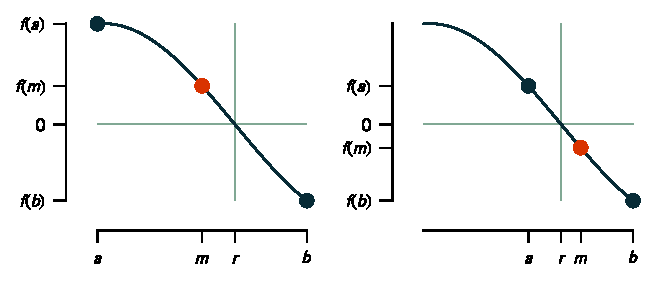
\includegraphics[width=\linewidth]{bisection-1}
\caption[First bisection step]{During the first iteration, we bisect the interval and determine whether the root of the function lies in $[a,m]$ or $[m,b]$.\label{f.bisection-1}}
\end{marginfigure}
A robust method for finding $x_{r}$ is \newterm{bisection}. We find the midpoint $m = (a+b)/2$ and compute $f(m)$ (red dot, Fig.~\ref{f.bisection-1}). We then determine the interval---$[a,m]$ or $[m,b]$ in which the root lies. For example, in Fig.~\ref{f.bisection-1}, the root lies in $[m,b]$ since $f(m)$ and $f(b)$ have opposite signs. We then reset the bounds of our interval---in this case, set $a=m$---and repeat the process (Fig.~\ref{f.bisection-2}).
\begin{marginfigure}
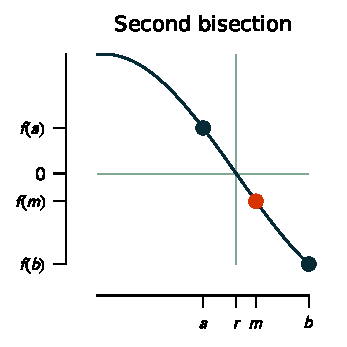
\includegraphics[width=\linewidth]{bisection-2}
\caption[Second bisection step]{For the second iteration, we move the left-boundary $a$ to $m$ and compute the next midpoint.\label{f.bisection-2}}
\end{marginfigure}

As shown in Fig.~\ref{f.bisection-2}, for the third iteration, we should set $b=m$. On each iteration the uncertainty in our root is halved: at the start the uncertainty is $\Delta=|b-a|$; after one iteration it is $\Delta/2$; after two iterations, $\Delta/2^{2}$; after $n$ iterations, $\Delta/2^{n}$. If our desired \newterm{tolerance} is $\epsilon$---that is, the root is known to lie in an interval of width $\epsilon$---then we should stop when
\begin{eqnarray*}
	\frac{\Delta}{2^{n}} &<& \epsilon\\
	n &>& \log_{2}\left(\frac{\Delta}{\epsilon}\right).
\end{eqnarray*}
Note the $\log_{2}$: on each iteration, we gain another bit of precision on the root. Since our precision is limited to roughly 52 bits (\S~\ref{s.numerical-precision}), in our code we could set the maximum number of iterations to, say, 60 and then exit the loop when $|b-a| < \epsilon$. The first five bisections for our example are shown in Fig.~\ref{f.bisection-3}.
\begin{marginfigure}
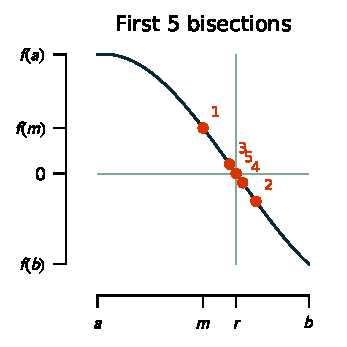
\includegraphics[width=\linewidth]{bisection-3}
\caption[First five bisections]{The first five bisections illustrating the convergence to the root.\label{f.bisection-3}}
\end{marginfigure}

\subsection{Newton's method}
Bisection is robust: it is guaranteed to converge to a root that is bracketed on some interval $a \le x \le b$. It converges to the root at a rather plodding pace, however, and you might wonder: can we do better? If we know the derivative of our function, $f^{\,\prime}(x)$, then we can use \newterm{Newton's method}. On each iteration $n$, with a trial root $x_{n}$, compute $f(x_{n})$ and $f^{\,\prime}(x_{n})$. Then compute the next guess for the root as
\[	x_{n+1} = x_{n} - \frac{f(x_{n})}{f^{\,\prime}(x_{n})}. \]
Fig.~\ref{f.newton} illustrates this: we equate the slope of the red dotted line, $(f(x_{0})-0)/(x_{0}-x_{1})$, with $f^{\,\prime}(x_{0})$ and solve for $x_{1}$. We then repeat this process to get $x_{2}$, $x_{3}$, and so on, with each one hopefully ever closer to the root.
\begin{marginfigure}
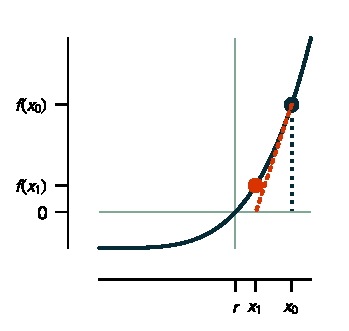
\includegraphics[width=\linewidth]{newton}
\caption[Schematic of Newton's method]{Starting from an initial guess $x_{0}$, we extend a line (red dotted line) of slope $f^{\,\prime}(x_{0})$ to where it crosses $y=0$, thus giving our next guess $x_{1}$.\label{f.newton}}
\end{marginfigure}

Compared with bisection, Newton's method converges quite rapidly: the precision roughly doubles on each iteration. Thus, for the example in Fig.~\ref{f.newton}, where $f(x) = x^{4}-4$ and $x_{0}=2$, only 6 iterations are needed to obtain the root to a tolerance $< 10^{-15}$. Nothing comes for free, however; if the initial guess is too far from the root, then Newton's method will converge very slowly or perhaps not at all (what happens if $x_{0}$ is near the left end of the curve in Fig.~\ref{f.newton}?).\marginnote{Newton's method is useful for quickly estimating roots of numbers: for example, to find the square root of a number $r$, start with a guess $x_{0}$ and compute $x_{1} = (x_{0}^{2} + r)/(2x_{0})$, then repeat to get $x_{2}$. Often one can do one or two iterations mentally and get within a percent or so. For example, to estimate $\sqrt{2}$: $x_{0} = 1$; $x_{1} = 3/2$; and $x_{2} = 17/12$, which is accurate to 0.2\%.}
For this reason, along with the need to compute the derivative, Newton's method is generally not preferred.

\subsection{Brent's method}
\newterm{Brent's method}\cite{Brent1973Algorithms-for-} is a rapidly converging, robust routine for finding roots. Like bisection, it requires that the root be bracketed on an interval $a\le x
\le b$; and like bisection, the initial guess for the root is the midpoint $m = (a+b)/2$. To construct the next guess for the root, Brent's method uses inverse quadratic interpolation: it fits a parabola $x = ay^{2}+ by + c$ through the three points $(a,f(a))$, $(m,f(m))$, and $(b,f(b))$.  This parabola crosses the line $y=0$ at $x=c$, and this is the next guess for the root. Solving for $c$ (see Box~\ref{sb.interpolation}) gives
\[
x = \frac{f(b)f(m)a}{[f(b)-f(a)][f(m)-f(a)]} - \frac{f(a)f(m)b}{[f(b)-f(a)][f(m)-f(b)]} 
        + \frac{f(a)f(b)m}{[f(m)-f(a)][f(m)-f(b)]}.
\]
Fig.~\ref{f.brent-1} illustrates this, using the same parameters as in Fig.~\ref{f.bisection-1}. The thin line shows the parabolic fit, and the red dot indicates the next guess $g$ for the root.
\begin{marginfigure}
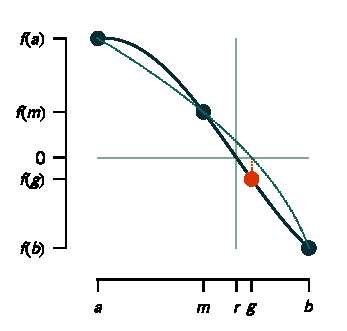
\includegraphics[width=\linewidth]{brent-1}
\caption[Brent's method]{A parabola $x=ay^{2}+by+c$ is fit through the ends and midpoint of an interval containing the root, and where this parabola intersects $y=0$---i.e., at $x=c$---is used as the next guess, labeled $g$, for the root.\label{f.brent-1}}
\end{marginfigure}

Because the root lies in $[m,b]$, for the next iteration (Fig.~\ref{f.brent-2}), we restrict the interval to $m\le x\le b$ and construct a parabola through the new left boundary $m$, the guess for the root $g$, and the right hand boundary $b$. After this second iteration, our new guess $g$ is quite close to the root; comparing with Fig.~\ref{f.bisection-3} illustrates how Brent's method is more efficient than bisection.
\begin{marginfigure}
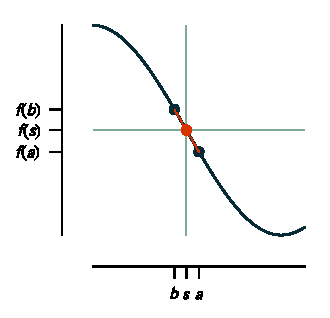
\includegraphics[width=\linewidth]{brent-2}
\caption[Second iteration, Brent's method]{Brent's method is repeated on the restricted interval $[m,b]$ using the points $m,g,b$ to fit a new parabola and determining the next guess (red dot) for the root.\label{f.brent-2}}
\end{marginfigure}

\begin{sidebar}[Interpolation]
\label{sb.interpolation}
Through any two points $(x_{0},y_{0})$, $(x_{1},y_{1})$ with $x_{1}\neq x_{0}$, we can fit a unique line, $y=ax+b$. The equation for a line has two undetermined coefficients, $a$ and $b$, and we find these coefficients by evaluating the equation for a line at each point:
\[
	y =  \frac{y_{2}-y_{1}}{x_{2}-x_{1}} x + \frac{y_{1}x_{2} - y_{2}x_{1}}{x_{2}-x_{1}}.
\]
Through any three points $(x_{0},y_{0})$, $(x_{1},y_{1})$, $(x_{2},y_{2})$ with $x_{0}\neq x_{1}\neq x_{2}$, we can fit a unique quadratic $q = ax^{2}+bx+c$, with $a,b,c$ determined by the equations
\begin{eqnarray*}
\left[\begin{array}{rrr}
1 & x_{0} & x_{0}^{2} \\
1 & x_{1} & x_{1}^{2} \\
1 & x_{2} & x_{2}^{2}
\end{array}\right] \left[\begin{array}{c} c\\b\\a\end{array}\right] = 
\left[\begin{array}{c} y_{0}\\y_{1}\\y_{2}\end{array}\right].
\end{eqnarray*}
Continuing, through 4 points we can fit a polynomial of degree 3: $p_{3}(x) = ax^{3} + bx^{2} + cx +d$; and so on. There is a formula for the polynomial of degree $N$, known as the \newterm{Lagrange polynomial}, that passes through $N+1$ points
\begin{eqnarray}
p_{N} &=& \sum_{i=0}^{N} y_{i}\ell_{i}(x),\\
\ell_{i}(x) &=& \prod_{k=0,k\neq i}^{N} \frac{x-x_{k}}{x_{i}-x_{k}}.
\end{eqnarray}
For example,
\begin{eqnarray}
p_{3}(x) =&&  y_{0}\frac{x-x_{1}}{x_{0}-x_{1}}\cdot\frac{x-x_{2}}{x_{0}-x_{2}}\cdot\frac{x-x_{3}}{x_{0}-x_{3}} \nonumber\\
      &+& y_{1}\frac{x-x_{0}}{x_{1}-x_{0}}\cdot\frac{x-x_{2}}{x_{1}-x_{2}}\cdot\frac{x-x_{3}}{x_{1}-x_{3}} \nonumber \\
      &+& y_{2}\frac{x-x_{0}}{x_{2}-x_{0}}\cdot\frac{x-x_{1}}{x_{2}-x_{1}}\cdot\frac{x-x_{3}}{x_{2}-x_{3}} \nonumber\\
      &+& y_{3}\frac{x-x_{0}}{x_{3}-x_{0}}\cdot\frac{x-x_{1}}{x_{3}-x_{1}}\cdot\frac{x-x_{2}}{x_{3}-x_{2}}.
\label{e.four-points}
\end{eqnarray}
\end{sidebar}

\section[Solving a system of ordinary differential equations]{Numerically solving a system of ordinary differential equations}
A common numerical task is to integrate a system of first-order ordinary differential equations (ODEs). That is, given a system of equations
\begin{equation}\label{e.equation}
\DDt{z} = f(t,z)
\end{equation}
with specified initial conditions $z(t=t_{0})$, find $z(t)$
Here $z$ is shorthand for an \emph{array} of variables: $z(t) = \{ z_{0}(t), z_{1}(t), z_{2}(t), \ldots\}$. Likewise, $f(t,z)$ is an array of known, specified functions: $f(t,z) = \{f_{0}(t,z), f_{1}(t,z), f_{2}(t,z), \ldots\}$.

An example is Newton's equation of motion,
\begin{equation}\label{e.Newton-2nd}
\frac{\dif^{2}\bvec{r}}{\dif t^{2}} = \frac{\bvec{F}}{m}.
\end{equation}
You may object that this is a second-order differential equation; but notice that if we define
\[
	\bvec{v} = \DDt{\bvec{r}}
\]
then we can recast this single second-order differential equation into a system of two\sidenote{Strictly speaking, this is a system of \emph{six} ODEs: three components of $\bvec{r}$ and three components of $\bvec{v}$.} first-order differential equations of the form (\ref{e.equation}):
\begin{eqnarray}
	\DDt{\bvec{r}} &=& \bvec{v}\\
	\DDt{\bvec{v}} &=& \frac{\bvec{F}}{m}.
\end{eqnarray}
An additional example is the system of first-order ordinary differential equations
\begin{eqnarray}
\DDt{z_{0}} &=&  2\pi z_{1}\label{e.z0}\\
\DDt{z_{1}} &=& -2\pi z_{0}\label{e.z1}
\end{eqnarray}
with boundary conditions
\begin{equation}\label{e.z-boundary}
	z_{0}(t=0) = 0,\qquad z_{1}(t=0) = 1.
\end{equation}
By taking the derivative of eq.~(\ref{e.z0}) with respect to $t$,
\[
	\DDt{}\DDt{z_{0}} = 2\pi\DDt{z_{1}} = -4\pi^{2} z_{0},
\]
and applying the boundary conditions (\ref{e.z-boundary}),
we find the solution to equations (\ref{e.z0})--(\ref{e.z1}):
\begin{eqnarray}
z_{0} &=& \sin(2\pi t),\label{e.z0-sol}\\
z_{1} &=& \cos(2\pi t).\label{e.z1-sol}
\end{eqnarray}
We'll now show how to obtain an approximate numerical solution for this system of ODEs.

\newthought{Suppose we know $z(t)$ at some point $t$} and we wish to make a numerical estimate of $z$ at a nearby point $t+h$. We have the values of $z$ and we can compute
\[
	\left.\DDt{z}\right|_{t} = f(t,z).
\]
We can implement $f(t,z)$ for equations~(\ref{e.z0})--(\ref{e.z1}) in a single function.

\begin{sidebar}[Functions]
What is a function in the context of a program? Basically, a function is a self-contained group of statements that you name. For example, to implement $\dif z/\dif t = f(t,z)$ for equations~(\ref{e.z0})--(\ref{e.z1}), we might write (in Python)
\begin{Verbatim}[numbers=none]
def f(t,z):
    """
    RHS of equation dz/dt = f(t,z)
    """
    # this makes an array of length 2,
    # each element of which is zero
    dzdt = np.zeros(2)

    # equation (A.5)
    dzdt[0] = 2.0*np.pi*z[1]
    # equation (A.6)
    dzdt[1] = -2.0*np.pi*z[0]
    return dzdt
\end{Verbatim}
In this listing we give our function the uninspired name \code{f}. A function may receive information, which is listed in the parentheses after the function name: \code{(t,z)}. Thus, the first line
\begin{Verbatim}[numbers=none]
def f(t,z):
\end{Verbatim}
says ``bundle the following list of statements together and call it \code{f}. The statements expect as input two variables, called \newterm{arguments}, which will be referred to in the function as \code{t} and \code{z}.''
This function then does three things: it creates an array \code{dzdt} of length 2, sets the first element of this array to \code{2.0*np.pi*z[1]}, and sets the second element to \code{-2.0*np.pi*z[0]}. The final statement
\begin{Verbatim}[numbers=none]
    return dzdt
\end{Verbatim}
says ``finish, and provide the value of \code{dzdt}'' to whatever \newterm{called} the function. Thus, for example, after defining the function, you could write
\begin{Verbatim}[numbers=none]
k = f(x,y)
\end{Verbatim}
where \code{x} and \code{y} are variables you had already defined.
Python would interpret this as: ``Execute the statements in the function \code{f}. In those statements, set the value of \code{t} to be that of \code{x} and the value of \code{z} to be that of \code{y}. After executing those statements, store the value of the function variable  \code{dzdt} in \code{k} and carry on.''
\end{sidebar}

With the definition of a function $f$, we can compute the right-hand side of equation~(\ref{e.equation}). Our problem can thus be stated as follows:
given $z(t)$, construct an estimate for $z(t+h)$. If we can do this, then we can advance the solution stepwise from the initial condition $z(t=t_{0})$. We'll now present three algorithms for doing so, starting with the least accurate. Our example will use $t=h=0.12$; Fig.~\ref{f.solution} shows the solution for $z_{0}(t)$ over this interval.
\begin{marginfigure}
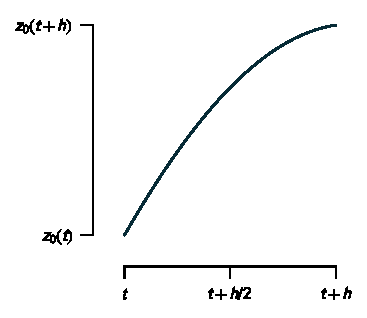
\includegraphics[width=\linewidth]{solution}
\caption[Solution for a sample set of ODE's]{\label{f.solution} Solution (\ref{e.z0-sol}) for $z_{0}$ in the system of equations (\ref{e.z0})--(\ref{e.z1}) from $t=0.12$ to $t+h=0.24$.}
\end{marginfigure}

\subsection{Forward Euler}

The first, and simplest, method goes back to Euler.
Suppose at time $t$ we know the solution $z(t)$ to eq.~(\ref{e.equation}). We can expand $z(t)$ as a Taylor series about this point to obtain
\[ z(t+h) = z(t) + h \left.\frac{\dif z}{\dif t}\right|_{t} + \frac{h^{2}}{2!} \left.\frac{\dif^{2} z}{\dif t^{2}}\right|_{t} + \ldots \]
But $\dif z/\dif t = f(t,z)$ is a known function. So to $\mathcal{O}(h^{2})$,
\begin{eqnarray}
	z(t+h) &\approx& z(t) + h \left.\frac{\dif z}{\dif t}\right|_{t}. \nonumber\\
		&=& z(t) + h \left.f(t,z)\right|_{t}.
\label{e.fEuler}
\end{eqnarray}
Figure \ref{f.forward-Euler} displays a schematic of a forward Euler step. We first compute the slope $f(t,z)$ and then use this to extend the solution to a point $t+h$. By repeating this step over and over, we can march our solution along.

\begin{figure}[htb]
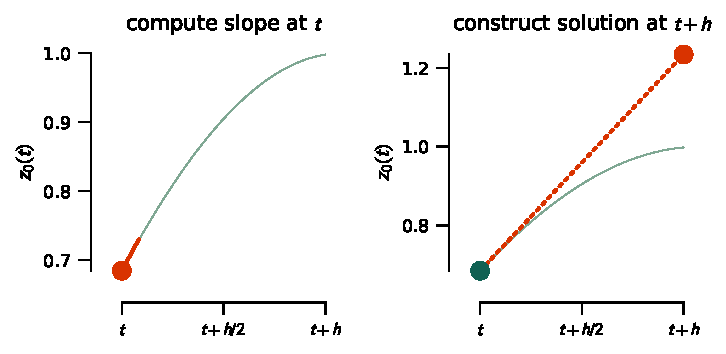
\includegraphics[width=\linewidth]{forward-Euler}
\caption{\label{f.forward-Euler}Schematic of a single forward Euler step.}
\end{figure}

How accurate is this \newterm{forward Euler} algorithm? From its definition, the error on each step comes from truncating the Taylor series and is $\mathcal{O}(h^{2})$. What do we mean by this? For sufficiently small $h$, reducing the step by a factor of 2 should reduce the error in a single step by a factor of 4. Another way to put this is that the forward Euler reproduces $z(t)$ exactly if $z$ is a linear function of $t$.
Unfortunately, errors tend to compound with each step, and the smaller the stepsize, the more steps are required. To integrate over a fixed interval $T$ takes $T/h$ steps; if the error on a given step is $\mathcal{E}\sim \mathcal{O}(h^{2})$, then the total integration error will be something like $T/h \times \mathcal{E} \sim \mathcal{O}(h)$.  We therefore call this forward Euler method a \textbf{first-order} method. Reducing the stepsize by a factor of 2 only reduces the integration error by a factor of 2.

\subsection{Second-order Runge-Kutta}

As you can see from Fig.~\ref{f.forward-Euler}, the forward Euler algorithm is not very accurate.
For the forward Euler method to be accurate, we must use a small step $h$ and therefore we must take many steps. We could be more efficient if our step agreed with the Taylor series to a higher order in $h$.

An improved method is to take, using forward Euler, a step to the midpoint of the interval,
\begin{equation}\label{e.predictor}
z_{\mathrm{P}}\left(t+\frac{h}{2}\right) = z(t) + \frac{h}{2}f[t,z(t)].
\end{equation}
Here $z_{\mathrm{P}}$ is our estimate of the solution at $t+h/2$.
\begin{figure}
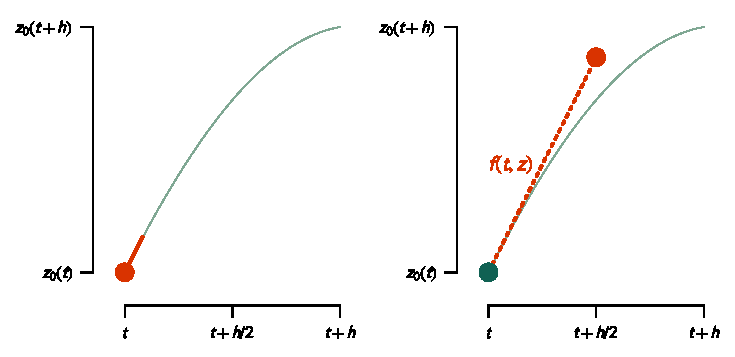
\includegraphics[width=\linewidth]{rk2-1}
\caption{First stage of a second-order Runge-Kutta step.}
\end{figure}

We then use $z_{\mathrm{P}}$ to get a better estimate of $f$ and use this corrected value of $f$ for a step across the entire interval:
\begin{equation}\label{e.corrector}
z(t+h) = z(t) + h f\left(t+\frac{h}{2},z_{\mathrm{P}}\right).
\end{equation}
\begin{figure}
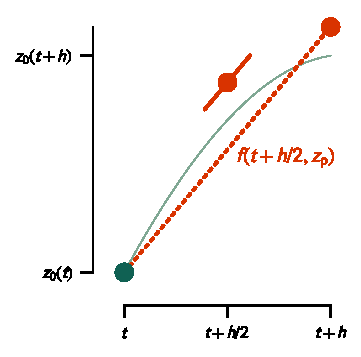
\includegraphics[width=\linewidth]{rk2-2}
\caption{Second stage of a second-order Runge-Kutta step.}
\end{figure}

One can show that $z(t+h)$ agrees with the actual solution to $\mathcal{O}(h^{3})$. When integrating over an interval $T$ and taking $T/h$ steps, the solution then has a global error $\sim\mathcal{O}(h^{2})$.  Equations~(\ref{e.predictor}) and (\ref{e.corrector}) are known as the \newterm{second-order Runge-Kutta} method. Note that if we reduce the stepsize by a factor of two, we expect the global truncation error to decrease by a factor of 4.

\subsection{Fourth-order Runge-Kutta}

An even better method is the classic \newterm{fourth-order Runge-Kutta} algorithm. In this method, the integration of $z$ from $t$ to $t+h$ is done in four steps. 

First, a trial forward Euler step is taken to the midpoint $t+h/2$ and the solution estimated there (Fig.~\ref{f.rk4-1}), just as in the second-order method.
\begin{figure}
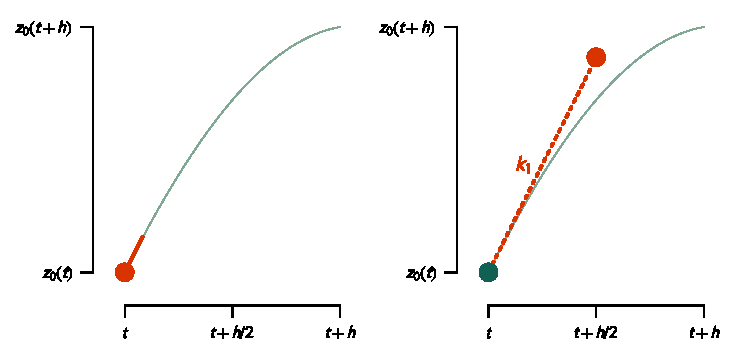
\includegraphics[width=\linewidth]{rk4-1}
\caption{First stage of a fourth-order Runge-Kutta step.\label{f.rk4-1}}
\end{figure}


This solution at the midpoint is used to make a better estimate of $f$, and a new step is taken, not to $t+h$, but rather from $t$ just to the midpoint $t+h/2$ again (Fig.~\ref{f.rk4-2}).
\begin{figure}
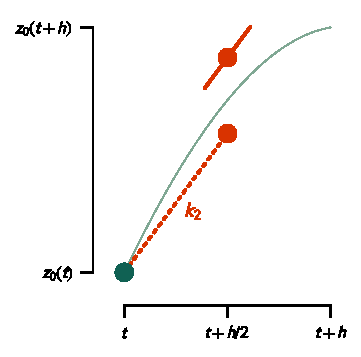
\includegraphics[width=\linewidth]{rk4-2}
\caption{Second stage of a fourth-order Runge-Kutta step.\label{f.rk4-2}}
\end{figure}

A new value of the slope $f$ at the midpoint is then computed, and this value of $f$ is then used to step across the full interval (Fig.~\ref{f.rk4-3}).
\begin{figure}
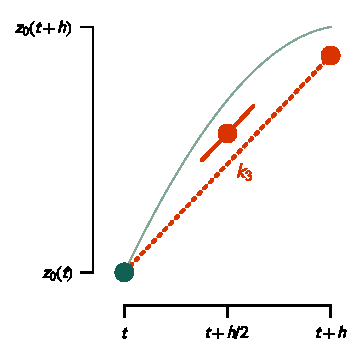
\includegraphics[width=\linewidth]{rk4-3}
\caption{Third stage of a fourth-order Runge-Kutta step.\label{f.rk4-3}}
\end{figure}

The slope at the endpoint $t+h$ is then computed. At this point, we have computed the following four estimates for the value of $\dif z/\dif t$:
\begin{eqnarray}
k_{1} &=& f(t,z(t)) \\
k_{2} &=& f\left(t+\frac{h}{2}, z(t) + \frac{h}{2}k_{1}\right)\\
k_{3} &=& f\left(t+\frac{h}{2},z(t) + \frac{h}{2}k_{2}\right)\\
k_{4} &=& f\left(t + h, z(t) + hk_{3}\right).
\end{eqnarray}
The solution $z(t+h)$ is then constructed from a weighted sum of the $k_{i}$ (Fig.~\ref{f.rk4-4}),
\begin{equation}\label{e.rk4}
	z(t+h) \approx z(t) + \frac{h}{6}\left(k_{1} + 2k_{2} + 2k_{3} + k_{4}\right).
\end{equation}
\begin{figure}
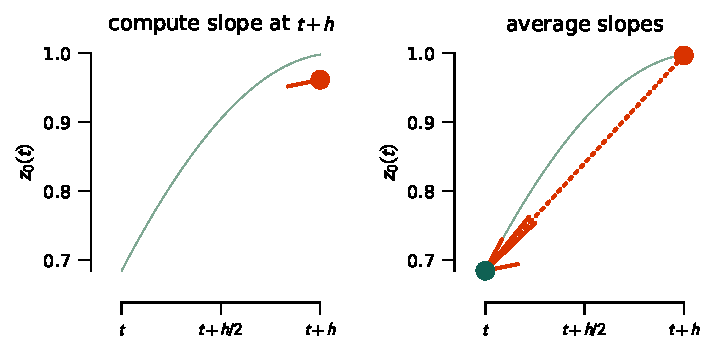
\includegraphics[width=\linewidth]{rk4-4}
\caption{Fourth and final stage of a fourth-order Runge-Kutta step.\label{f.rk4-4}}
\end{figure}

Notice that the $k_{i}$ are not independent of one another: each one depends on the intermediate value of $z$ computed in the previous step. The fourth-order Runge-Kutta scheme ``sniffs'' the behavior of $f(t,z)$ over the interval $(t,t+h)$ and constructs a weighted approximation for $\dif z/\dif t$.  One can show that this method produces solutions with a global truncation error $\sim\mathcal{O}(h^{4})$. That is, reducing the stepsize by a factor of 2 should reduce the error by a factor $2^{4} = 16$.

\section{Cubic splines}
As discussed in Box~\ref{sb.interpolation}, a common numerical task is to interpolate values in a data file. In stellar physics, this is often done for opacities or equation of state: one computes, or measures, the opacity under a limited set of composition, temperature, and density. From this table, we then interpolate to obtain values of the opacity at arbitrary conditions. There are many tradeoffs in how this interpolation is done. In this section we'll illustrate one such method, namely cubic splines.

\begin{marginfigure}
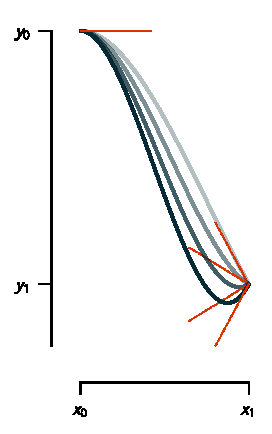
\includegraphics{spline-1}
\caption{\label{f.spline-1}Cubic polynomials between points $(x_{0},y_{0})$ and $(x_{1},y_{1})$; the slope at $x_{0}$ is $k_{0}=0$, and the slope $k_{1}$ is varied (red dotted lines).}
\end{marginfigure}
Through any 4 points $(x_{i},y_{i})_{i=0,\ldots,3}$ we can fit a unique cubic polynomial $y=p_{3}(x)$ (eq.~[\ref{e.four-points}]).  Alternatively, we can fit a cubic polynomial between two points $(x_{i},y_{i})$ and $(x_{i+1},y_{i+1})$ if we also specify the first derivatives $k_{i}$ and $k_{i+1}$ at $x_{i},x_{i+1}$: define $m_{i} = (y_{i+1}-y_{i})/(x_{i+1}-x_{i})$ as the mean slope across the interval; then the cubic polynomial is
\begin{eqnarray}
\lefteqn{q_{i}(x) =   y_{i}\frac{x_{i+1}-x}{x_{i+1}-x_{i}} 
		   + y_{i+1}\frac{x-x_{i}}{x_{i+1}-x_{i}}
		   + \frac{(x-x_{i})(x_{i+1}-x)}{x_{i+1}-x_{i}}} && \nonumber\\
		   && \times\left[\frac{x_{i+1}-x}{x_{i+1}-x_{i}}(k_{i}-m_{i})
		       -\frac{x-x_{i}}{x_{i+1}-x_{i}}(k_{i+1}-m_{i})\right].
\label{e.spline}
\end{eqnarray}
An example of a cubic between $(x_{0},y_{0})$ and $(x_{1},y_{1})$ with $k_{0}=0$ and various $k_{1}$ is shown in Fig.~\ref{f.spline-1}.

\begin{exercisebox}
Verify that $q_{i}(x_{i}) = y_{i}$ and $q_{i}(x_{i+1}) = y_{i+1}$; also verify that $q^{\prime}_{i}(x_{i}) = k_{i}$ and $q^{\prime}_{i}(x_{i+1}) = k_{i+1}$.
\end{exercisebox}

Now suppose we have a sequence of $N+1$ points $x_{0},x_{1},\ldots,x_{N}$ with data values $y_{0},y_{1},\ldots,y_{N}$. On each interval $[x_{i},x_{i+1}]$ we can construct a spline $q_{i}$. As an example, we take one of the curves from Fig.~\ref{f.spline-1} and cut it in two. We then clamp the derivatives at the endpoints and allow the first derivative at the interior point to vary, with the requirement that the first derivative is continuous at that point. 
\begin{marginfigure}
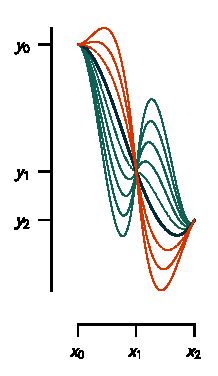
\includegraphics{spline-2}
\caption{\label{f.spline-2} Two splines spanning $[x_{0},x_{1}]$ and $[x_{1},x_{2}]$. The slope at the inner point, $k_{2}$, is allowed to vary. The dark curve shows the case where the first derivative is fixed to the value from original spline shown in Fig.~\ref{f.spline-1}.}
\end{marginfigure}

As the slope at $x_{1}$ is varied, the splines to left and right become more tortuous. This tight bending is characterized by the second derivative of the spline. In Fig.~\ref{f.spline-3} we plot the second derivative for three cases: where $k_{1}$ is fixed to the value from the original spline (solid line), and cases from Fig.~\ref{f.spline-2} with $k_{1}$ less than (dashed line) and greater than (dotted line) this value. Note that in general the second derivative is not continuous at $x_{1}$. 

\begin{marginfigure}
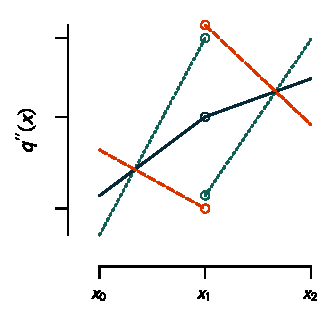
\includegraphics[width=\linewidth]{spline-3}
\caption{\label{f.spline-3} Second derivatives of our spline functions.}
\end{marginfigure}

Thus, we can generate a smooth curve by requiring that both the first and second derivatives be continuous at the junction points $x_{1},\ldots,x_{N-1}$. Let's check if this gives us enough conditions. For $N+1$ points $x_{0},x_{1},\ldots,x_{N}$ with data values $y_{0},y_{1},\ldots,y_{N}$, there are $N$ splines: $q_{0}(x)$ on $x_{0}\le x\le x_{1}$, $q_{1}(x)$ on $x_{1}\le x \le x_{n}$, and on to $q_{N-1}(x)$ on $x_{N-1}\le x\le x_{N}$. Each spline has 4 free parameters, so we have a total of $4N$ parameters. We have the following conditions:
\begin{eqnarray*}
q_{i}(x_{i}) &=& y_{i},\;i=0,\ldots,N-1\qquad\textrm{($N$ conditions)}\\
q_{i}(x_{i+1}) &=& y_{i+1},\;i=0,\ldots,N-1\qquad\textrm{($N$ conditions)}\\
q^{\prime}_{i}(x_{i}) &=& q^{\prime}_{i-1}(x_{i}),\;i=1,\ldots,N-1\qquad\textrm{($N-1$ conditions)}\\
q^{\prime\prime}_{i}(x_{i}) &=& q^{\prime\prime}_{i-1}(x_{i}),\;i=1,\ldots,N-1\qquad\textrm{($N-1$ conditions)}.
\end{eqnarray*}
Our format of the spine, eq.~(\ref{e.spline}), automatically satisfies the first two of these. Adding in the continuity of the first and second derivatives brings us to a total of $4N-2$ equations, and leaves us with two free parameters, namely $k_{0}$ and $k_{N}$, the derivatives at then ends. We could specify them (known as a \newterm{clamped spline}), but we usually don't have any way of knowing them \emph{a priori}. A popular choice is to set the second derivative at $x_{0}$ and $x_{N}$ to zero (known as a \newterm{natural} spline).\marginnote{A third choice is the \newterm{not-a-knot} condition, in which we also require the \emph{third} derivative at $x_{1}$ and $x_{N-1}$ to be continuous.}

Let's consider the case of a natural spline. Taking the second derivative of eq.~(\ref{e.spline}) and substituting $x=x_{i}$ and $x=x_{i+1}$ gives
\begin{eqnarray}
\label{e.d2spline-left}
q^{\prime\prime}_{i}(x_{i}) &=& -\frac{2}{x_{i+1}-x_{i}}\left[ 2k_{i} + k_{i+1} - 3m_{i} \right];\\
\label{e.d2spline-right}
q^{\prime\prime}_{i}(x_{i+1}) &=& \frac{2}{x_{i+1}-x_{i}}\left[ k_{i} + 2k_{i+1} - 3m_{i} \right].
\end{eqnarray}
Defining $\Delta_{i} = (x_{i+1}-x_{i})^{-1}$ and equating second derivatives at the interior points $x_{i},\,i=1,\ldots,N-1$ then yields the following $N-1$ equations for the $k_{i}$, $i=1,\ldots,N-1$:
\begin{equation}
\Delta_{i-1}k_{i-1} + 2\left(\Delta_{i-1} + \Delta_{i}\right) k_{i} + \Delta_{i}k_{i+1} = 3\left(m_{i-1}\Delta_{i-1} + m_{i}\Delta_{i}\right)
\end{equation}
Setting the second derivatives to zero at $x_{0}$, $x_{N}$ gives the additional equations
\begin{eqnarray}
2k_{0} + k_{1} &=& 3m_{0}\\
k_{N-1} + 2k_{N} &=& 3m_{N-1}.
\end{eqnarray}
These $N+1$ equations for the $N+1$ $k_{i}$ can be written as the matrix equation
\[
\left[\begin{array}{ccccccccccc}
	b_{0} & c_{0} \\
	a_{1} & b_{1} & c_{1} \\
	& a{2} & b_{2} & c_{2}\\
	& & \ddots & \ddots & \ddots \\
	& & & a_{i} & b_{i} & c_{i} \\
	& & & & \ddots & \ddots & \ddots \\
	& & & & & a_{N-1} & b_{N-1} & c_{N-1} \\
	& & & & & & a_{N} & b_{N} 
\end{array}\right]
\left[\begin{array}{c}
	k_{0}\\
	k_{1}\\
	k_{2}\\
	\vdots\\
	k_{i}\\
	\vdots\\
	k_{N-1}\\
	k_{N}
\end{array}\right] = 
\left[\begin{array}{c}
	d_{0}\\
	d_{1}\\
	d_{2}\\
	\vdots\\
	d_{i}\\
	\vdots\\
	d_{N-1}\\
	d_{N}
\end{array}\right].
\]
This is a \newterm{tridiagonal} matrix equation, and is easily solved.